\documentclass[../main/main.tex]{subfiles}


\begin{document}

\section{March 9th, 2021}
\subsection{Convergence of Steepest Descent}
\begin{theorem}
  Let $A \in \RR ^{n\times n}$ be SPD. Then $\{x_{k}\}$ generated by steepest descent satisfies: \[
\|x_{k+1}-x_{*}\|_{A} \leq \frac{\gamma -1}{\gamma +1} \|x_{k}-x_{*}\|_{A}
  \]  where: $\gamma  = \frac{\lambda _{\max }(A)}{\lambda _{\min }(A)} $ is the condition number of $A$.
\end{theorem}
  \begin{proof}
    Due to the optimality of $x_{k+1}$: \begin{align*}
                                          \|x_{k+1}-x_{k}\|_{A} &= \min _{x\in x_{k}+\sspan \{r_{k}\}} \|x-x_{*}\|_{A}\\
                                                                &= \min _{\beta \in \RR }\|(x_{k}-\beta r_{k})- x_{*}\|_{A}\\
                                                                &=\min _{\beta \in \RR }\|(x_{k}-x_{*})+\beta A(x_{k}-x_{*})\| _{A} \\
                                                                &=\min _{p\in \mathbb{P}_{1}, p(0)=1} \|p(A)\cdot (x_{k}-x_{*})\|_{A}
                                                                &\leq \left(\min _{p\in \mathbb{P}_{1}, p(0)=1} \|p(A)\|_{A}\right) \|x_{k}-x_{*}\|_{A}
                                          .\end{align*}
                                        Where $\mathbb{P}_{1} $ is the set of all polynomial of degree 1. Note that minimizing over $\beta $ is minimizing over $\mathbb{P}_{1}$ where $p(0)=1$, since we can take $\{1+\beta t : \beta \in \RR \}$.
  \begin{lemma}
    Let $B\in \RR ^{n\times n}$. Then: \[
      \|B\|_{A} = \|A^{\frac{1}{2}}B A^{-\frac{1}{2}}\|_{2}
    \] where $A^{\frac{1}{2}}$ is the square root of $A$ (using eigenvalue decomposition).
  \end{lemma}
  \begin{proof}
    \[
      \|B\|_{A}^2 = \max _{x\in \RR ^{n}} \frac{\iprod{ABx}{Bx}}{\iprod{Ax}{x}}  = \max_{y\in \RR ^{n}} \frac{\iprod{A^{\frac{1}{2}}BA^{-\frac{1}{2}}y}{A^{\frac{1}{2}}B A^{\frac{1}{2}}y}}{\iprod{y}{y}}  = \|A^{\frac{1}{2}}B A^{-\frac{1}{2}}\|^2_{2}
    \] where $y=A^{\frac{1}{2}}y \iff x = A^{-\frac{1}{2}}y$
  \end{proof}
  Then \[\ |p(A)\|_{A} = \|A^{\frac{1}{2}}p(A)A^{-\frac{1}{2}}\|_{2}= \|p(A)\|_{2} = \max _{i=1, \ldots  ,}|p(\lambda_{i})|,
  \] where $\lambda _{i}$ are eigenvalues of $A$. Therefore:
  \begin{align*}
    \|x_{k+1}-x_{*}\|_{A} &\leq  \left(\min _{p\in \mathbb{P}_{1}, p(0)=1}\|p(A)\|_{A}\right)\|x_{k}-x_{*}\|_{A} \\
&\leq  \left(\min _{p\in \mathbb{P}_{1}, p(0)=1} \max_{i=1, \ldots ,n}|p(\lambda_{i})|\right)\|x_{k}-x_{*}\|_{A} \\
&\leq  \left(\min _{p\in \mathbb{P}_{1}, p(0)=1} \max_{\lambda \in [\lambda_{\min },\lambda_{\max }]}|p(\lambda)|\right)\|x_{k}-x_{*}\|_{A}
    .\end{align*}
  \begin{remark}
This is taking the infinity norm, which will be discussed in further detail later.
  \end{remark}
  This minimax occurs when: \[
    |p(\lambda_{\min })| = |p(\lambda_{\max }) \text{ and }p\left(\frac{\lambda _{\min }+\lambda _{\max }}{2} \right) \implies  p(t) = 1- \frac{2}{\lambda _{\min }+\lambda _{\max }}t
  \] Thus: \[
\min _{p\in \mathbb{P}_{1}, p(0)=1} \max_{\lambda \in [\lambda_{\min },\lambda_{\max }]}|p(\lambda)| = 1- \frac{2}{\lambda _{\min }+\lambda _{\max }}\lambda _{\min } = \frac{\lambda _{\max }- \lambda _{\min }}{\lambda _{max}+\lambda _{\min }} = \frac{\gamma -1}{\gamma +1}
  \]
  \end{proof}
  \begin{remark}
Thus, the convergence speed is $\frac{\gamma -1}{\gamma +1} $.
  \end{remark}
  To achieve an $\epsilon $-solution, it suffices to have: \[
    \left(\frac{\gamma -1}{\gamma +1} \right)^{k}\|x_{0}-x_{*}\|_{A}\leq \epsilon  \implies  k \log \left(\frac{\gamma -1}{\gamma +1} \right)\leq  \log \left(\frac{\epsilon }{\|x_{0}-x_{*}\|_{A}} \right) \implies k\geq \frac{\log\left(\frac{\|x_{0}-x_{*}\|_{A}}{\epsilon } \right)}{\log \left(\frac{\gamma +1}{\gamma -1} \right)}
  \]
  Because: \[
\log \left(\frac{\gamma +1}{\gamma -1} \right)= \log \left(1+\frac{2}{\gamma -1}\right)\approx \frac{2}{\gamma } \text{ if $\gamma $ is large}.
\]Thus, we have: \[
  k \geq   \frac{1}{2} \log \left( \frac{\|x_{0}-x_{*}\|_{A}}{\epsilon } \right) \cdot \gamma
\]
\begin{remark}
The number of iterations needed is $O(\gamma)$.
\end{remark}
\subsection{Two-Dimensional Projection Method (Conjugate Gradient)}
We consider the projection method where $\dim(K)=2$. We choose: \[
  K=\sspan \{r_{k},\, d_{k-1}\}
\] where: \[
\begin{cases}
  r_{k} = b-Ax_{k} &\text{ (potential) }\\
  d_{k-1} = x_{k-1}-x_{k} &\text{ (momentum) }
\end{cases}
\]
A pictorial representation of this is given in Fig \ref{fig:3-9-proj}.
\begin{figure}[htpb]
  \centering
  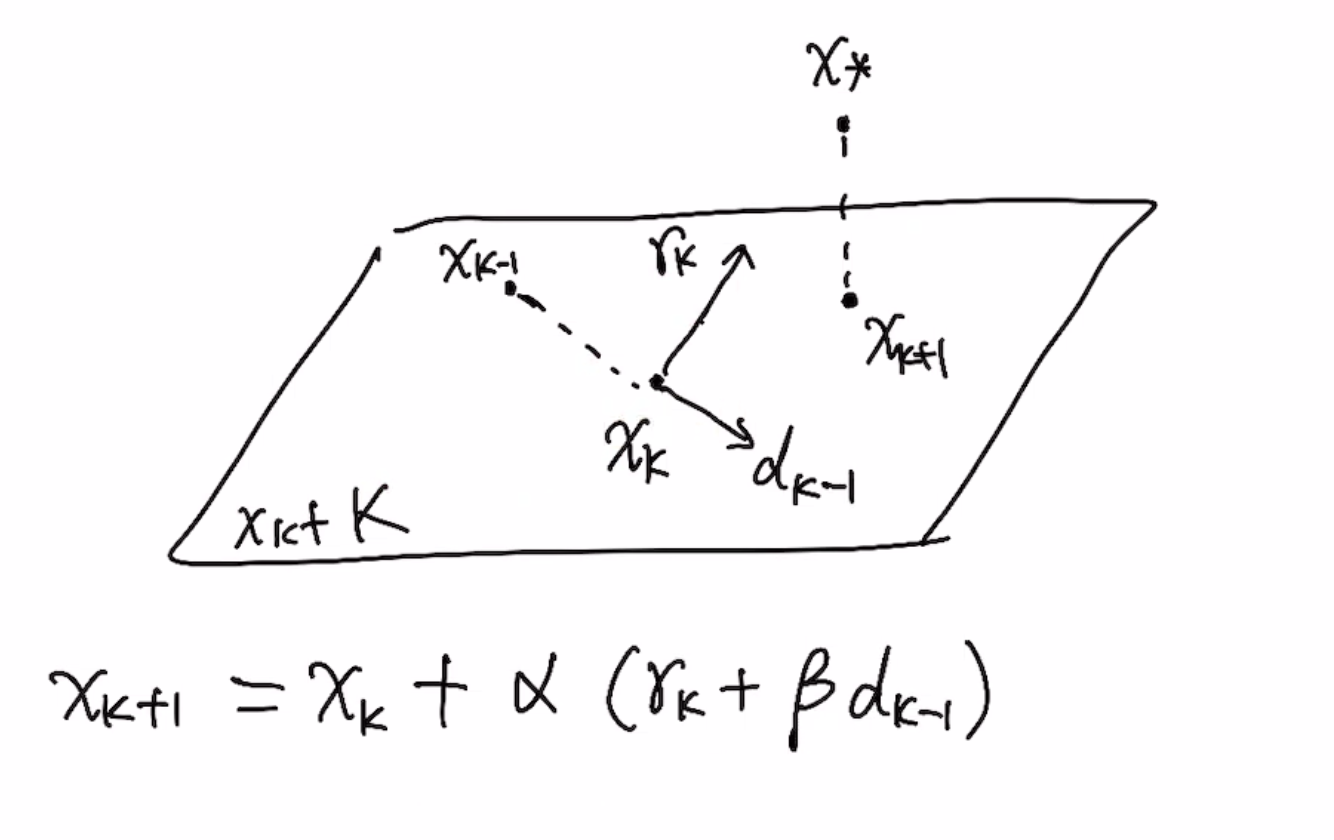
\includegraphics[width=0.7\textwidth]{../images/3-9-proj}
  \caption{Pictorial Representation of $x_{k}+K$}
  \label{fig:3-9-proj}
\end{figure}
\begin{remark}
Recall that $r_{k}$ is the best possible direction in 1D.
\end{remark}
Thus, we have: \[
  x_{k+1} = x_{k} + \alpha_{k}  (r_{k}+\beta_{k} d_{k-1}), \quad  \text{where }\alpha _{k},\beta _{k} \in \RR
\] with: \[
  (\alpha_{k},\beta_{k}) = \argmin_{\alpha ,\beta\in \RR } \|x_{k}+\alpha (r_{k}+\beta d_{k-1})-x_{*}\|^2_{A}
\]
Now we find the expressions of $\alpha _{k}, \beta _{k}$: \begin{align*}
                                                            \|x_{k}+\alpha (r_{k}+\beta d_{k-1})-x_{*}\|^2_{A} &=\|x_{k}-x_{*}\|^2_{A} + 2\alpha \iprod{x_{k}-x_{*}}{r_{k}}_{A}+\alpha ^2 \|r_{k}\|^2_{A} \\
                                                            &\quad  + 2\alpha \beta \iprod{x_{k}-x_{*}}{d_{k-1}}_{A}+\alpha ^2\beta ^2\|d_{k-1}\|_{A}^2 + 2\alpha ^2\beta \iprod{r_{k}}{d_{k-1}}_{A} .\end{align*}
                                                          Because $x_{k}$ is the projection of $x_{*}$ onto $x_{k-1}+\sspan \{r_{k-1},d_{k-2}\}$, we have: \[
                                                            \iprod{x_{k}-x_{*}}{d_{k-1}}_{A} = 0\]Taking derivative w.r.t $\alpha,\beta $ and setting them to 0, we have: \[
\begin{cases}

  2\iprod{x_{k}-x_{*}}{r_{k}}_{A}+2\alpha _{k}\|r_{k}\|^2_{A}+2\alpha _{k}\beta _{k}^2 \|d_{k-1}\|^2_{A}+4 \alpha _{k}\beta _{k}\iprod{r_{k}}{d_{k-1}}_{A} = 0\\
  2\alpha _{k}^2 (\beta_{k}\|d_{k-1}\|_{A}^2 +2\iprod{r_{k}}{d_{k-1}}_{A}) = 0
\end{cases}
\]
\begin{itemize}
\item If $\alpha_{k}=0$, then: $x_{k+1}=x_{k}$ = projection of $x_{*}$ onto $x_{k}+\sspan \{ r_{k}, d_{k-1}\}, $ \begin{align*} &\iff  \iprod{x_{*}-x_{k}}{r_{k}}_{A}=0 \\
                                                                                                              &\iff  \iprod{r_{k}}{r_{k}}=0 \\
                                                                                                              &\iff  r_{k} = 0 \iff  Ax_{k} = b \\
                                                                                                              &\iff  x_{k} = x_{*} .\end{align*}
         $x_{k}$ is the exact solution, and the algorithm stop.
  \item If $\alpha _{k}\neq 0$, then $r_{k}\neq 0$ and: \[
\beta _{k} = -\frac{\iprod{r_{k}}{d_{k-1}}_{A}}{\|d_{k-1}\|_{A}^2}
        \]
\end{itemize}
Then denote $d_{k}=r_{k} + \beta _{k}d_{k-1}$. So:
\begin{align*}
  &\alpha _{k} = \argmin _{\alpha \in \RR } \|(x_{k}+\alpha d_{k})-x_{*}\|_{A}\\
  \iff &\alpha _{k}=\argmin_{\alpha \in \RR }\|x_{k}-x_{*}\|_{A}^2 + 2\alpha \iprod{d_{k}}{x_{k}-x_{*}}_{A}+\alpha ^2\|d_{k}\|_{A}^2
  .\end{align*}
Taking the derivative and setting to zero, we have:
\begin{align*}
  &2\alpha _{k}\|d_{k}\|_{A}^2 = -2 \iprod{d_{k}}{x_{k}-x_{*}}_{A}\\
  \iff &\alpha _{k}= -\frac{\iprod{d_{k}}{x_{k}-x_{*}}_{A}}{\|d_{k}\|_{A}^2} = - \frac{\iprod{d_{k}}{-r_{k}}}{\iprod{Ad_{k}}{d_{k}}}  \\
  \iff & \alpha _{k} = \frac{\iprod{d_{k}}{r_{k}}}{\iprod{Ad_{k}}{d_{k}}}
  .\end{align*}

Thus, we have Algorithm \ref{3-9-alg}.
        \begin{algorithm}[h!]
	\caption{Conjugate Gradient Method}
    \label{3-9-alg}
	\begin{algorithmic}[1]
    \State $d_{-1}=0$
      \For{ $k=0,1,2, \ldots$}
      \State $r_{k}=b-Ax_{k}$
      \State $\beta _{k} = - \frac{\iprod{r_{k}}{Ad_{k-1}}}{\iprod{d_{k-1}}{Ad_{k-1}}} $
      \State $d_{k}= r_{k}+\beta _{k}d_{k-1}$
      \State $\alpha _{k} = \frac{\iprod{d_{k}}{r_{k}}}{\iprod{Ad_{k}}{d_{k}}} $
      \State $x_{k+1} = x_{k} +\alpha _{k}d_{k}$
      \EndFor
	\end{algorithmic}
	\end{algorithm}

Algorithm \ref{3-9-alg} requires 2 matrix-vector products + operations of $O(n)$. It can be improved to only requiring one matrix vector product, similarly to before, by introducing: \[
  p_{k} = Ad_{k}.
\] Then we have:
\begin{align*}
  Ax_{k+1} &= Ax_{k} + \alpha _{k}A d_{k}\\
  (b-Ax_{k+1})&=(b-Ax_{k})-\alpha _{k}Ad_{k}\\
 r_{k+1} &= r_{k}-\alpha _{k}p_{k}
  .\end{align*}
        \begin{algorithm}[h!]
	\caption{2D Projection Method Improved}
    \label{3-9-alg2}
	\begin{algorithmic}[1]
    \State $d_{-1}=0$
    \State $p_{-1}=0$
    \State $r_{0}=b-Ax_{0}$
      \For{ $k=0,1,2, \ldots$}
      \State $\beta _{k} = - \frac{\iprod{r_{k}}{p_{k-1}}}{\iprod{d_{k-1}}{p_{k-1}}} $
      \State $d_{k}= r_{k}+\beta _{k}d_{k-1}$
      \State $p_{k} = Ad_{k}$
      \State $\alpha _{k} = \frac{\iprod{d_{k}}{r_{k}}}{\iprod{p_{k}}{d_{k}}} $
      \State $x_{k+1} = x_{k} +\alpha _{k}d_{k}$
      \State $r_{k+1}=r_{k}-\alpha _{k}p_{k}$
      \EndFor
	\end{algorithmic}
	\end{algorithm}

  \begin{remark}
Algorithm \ref{3-9-alg2} only requires 1 matrix-vector product and opeartions of $O(n)$.
  \end{remark}
\begin{definition}
Algorithm \ref{3-9-alg2} is called the \vocab{Conjugate Gradient (CG)} method. \index{conjugate gradient}
\end{definition}
Recall that the CG method is an optimization algorithm for: \[
\min _{x\in \RR ^{n}}f(x), \quad  f(x) = \frac{1}{2} x^{T}Ax - x^{T} b.
\] For this problem, we have shown a few different variations of gradient descent:
\begin{itemize}
        \item (with exact line search) gives us Steepest Descent.
        \item (accelerated by momentum) gives us SOR Method.
        \item (simultaneously apply momentum and potential) gives us CG Method.
        \item (successively apply momentum then potential) gives us the \vocab{Nesterov momentum algorithm}. \index{Nesterov momentum algoritm}
        \item (successively apply potential then momentum) gives us gradient descent but with a larger step size (not optimal, which is exact line search).
\end{itemize}
For quadratic function $f(x)$ of the form \[
f(x) = \frac{1}{2} x^{T}Ax - x^{T} b,
\] CG is preferred. For general non-linear function, Nesterov is preferred because $\alpha _{k}$ and $\beta _{k}$ are not easy to obtain in CG. As such, Nesterov is popular in machine learning due to the complex objective function.

\begin{remark}
  If $f(x)$ is quadratic, we can get the optimal $\alpha _{k}$ and $\beta _{k}$, allowing us to update them simultaneously in CG.
\end{remark}
\begin{remark}
Best NN optimization function is probably just SGD with Nesterov acceleration.
\end{remark}
\end{document}
